\cotefile{40}
\scanpage{16}
% L1
Il faut \unsure{prouver} alors que, posant
% L2
\[
g_{\unsure{C|c}}=\unsure{\gamma|\rho}\circ\psi'_1
  \colon B\mathrel{\unsure{\text{\textemdash}|\longrightarrow}}C\otimes C
\]
% L3
\margin{\uline{???}}l'hom $g_C$ satisfait les relations (i) et (ii).

% L4
Pour ceci, \textendash\ \textendash\ \textendash\ \textendash
% archive sheet number: 15
\scanpage{17}
% L1–2
Considérons l'hyperalgèbre
\[
\unsure{\mathcal U|U}=A[X]/X^pA[X]
\]
% L3–4
sur l'anneau $A$ \inserted{de car.~$p$}, avec $\Delta$ donné par
\[
\boxed{\Delta X=X\otimes1+1\otimes X}
\]
% L5–8
[\,cela définit à priori $A[X]\mathrel{\unsure{\text{\textemdash}|\longrightarrow}}A[X]\otimes A[X]$, mais
$\Delta X^p=X^p\otimes1+1\otimes X^p$ est \unsure{appliqué|multiple} sur l'idéal
$A[X]\otimes X^pA[X]+X^pA[X]\otimes A[X]$\,], l'augmentation étant définie par
\deleted{\unsure{l'augmentation|l'image}} $\boxed{\varepsilon(X)=0}$, et le $\vee$ par $\boxed{\overset{\vee}{X}=-X}$

% L9–12
Cette hyperalgèbre est isomorphe à sa duale, \deleted{à l'aide}
On la regarde comme \deleted{\unsure{l'anneau des opérateurs|l'algèbre des opérateurs}} dual d'un groupe dans la catégorie des $A$-algèbres commutatives.

% L13–16
Soit $C$ une $A$-algèbre commutative. \unsure{De|Le|La|Se} faire opérer l'hyperalgèbre $\mathcal U$ sur $C$ revient à définir l'image $\deleted{X}\unsure{D'|D^{1}|D}$ de $\deleted{D}X$, i.e. à se donner un opérateur $D$ $A$-linéaire de $C$. De plus
% L17–18
\[
D^p=0\tag*{(i)}
\]
(exprime que $D$ définit une représentation de $A$-algèbre de $A[X]/X^pA[X]$ ds $\unsure{L_A|\mathcal L_A}(C,C)$)
% L19–20
\[
D(xy)=xDy+yDx\tag*{(ii)}
\]
(exprime que cette représentation est compatible avec $\Delta$)

% L21–22
donc \unsure{tt} revient à la \uline{donnée d'une $A$-dérivation} de puissance \unsure{$p^{\text{ième}}$|$p$-ième} nulle.

% L23–27
On veut exprimer maintenant que $C$ est un $\deleted{\unsure{U|H}}\unsure{U'|\mathcal U'|B|B'}$-espace \uline{principal} \uline{homogène} dans la catégorie des $A$-algèbres commutatives. On suppose \deleted{d'abord que} déjà que $C$ \deleted{\unsure{admet une}} \inserted{est \deleted{\unsure{lib|libre}}} un $A$-module libre (c'est sensiblement une
% archive sheet number: 16
\scanpage{18}
% L1–4
conséquence de notre hypothèse), et \deleted{\unsure{que}} son rang sera nécessairement $p$. Ceci dit il faut exprimer que les $D^i$ $(0\leq i\leq p-1)$ forment une \uline{base} du $\unsure{K|C|k}$-module $\operatorname{Hom}_A(C,C)$ [où on pose $(\lambda u)(\unsure{\mu|\rho|y})=\lambda(u(\mu))$].

% L5
\deleted{Soit p.ex.}

% L6–8
Supposons p.ex. que $C$ admette une $p$-base \inserted{sur $A$} réduite à un élément $u$, donc \unsure{on a|que}
\[
C\simeq A[u]/(u^p-a),\qquad\text{où }a\in A.
\]
\deleted{Posons} \deleted{\unsure{Donc|$Du$}} Alors une $A$-dérivation de $C$ est connue quand on connaît sa valeur sur $u$, qui peut-être choisie arbitrairement.

% L12–14
Définissons alors la $A$-dérivation $D$ dans $C$ par
\[
\begin{aligned}
&Du=1\\
\text{d'où}\qquad &Du^n=nu^{n-1}
\end{aligned}
\]
% L15–19
On a donc $D^p=0$, donc $C$ est un $\deleted{\unsure{D}}\unsure{U|\mathcal U}$-module. De plus, \deleted{la matrice des} identifions, grâce à la base $(u^i)_{0\leq i\leq p-1}$, \deleted{\unsure{le|et}} $\operatorname{Hom}(C,C)$ à $C^p$, par $v\mathrel{\unsure{\text{\textemdash}|\longrightarrow|\mapsto}}(v(u^i))_{\unsure{0\leq i\leq p-1}}$ [c'est un isom. de $C$-modules]. Alors
% L20–21
la matrice du système des $D^i$ $(0\leq i\leq p-1)$ est
\[
\left(\begin{array}{ccccc||l}
1&&u&u^2&u^3&u^{p-1}\\
0&&1&2u&3u^2&(p-1)u^{p-2}\\
0&&0&2.1&3.2.u&(p-1)(p-2)u^{p-3}\\
0&&0&0&3.2.1.&(p-1)(p-2)(p-3)u^{p-4}\\ \cline{2-6}
0&0&0&0&0&(p-1)\cdots1.
\end{array}\right)
\]
% archive sheet number: 17
\scanpage{19}
% L1–2
Son déterminant est égal à
\[
0!\;1!\;2!\;\unsure{\text{\textemdash}|\ldots|\cdots}\;(p-1)!
\]
% L3–6
qui provient donc d'un élément non nul de $\mathbb Z/pZ$, donc est inversible dans $C$, i.e. les $D^i$ $(0\leq i\leq p-1)$ forment bien une base de $\operatorname{Hom}_{\unsure{,|A}}(C,C)$ sur $C$. Donc

% L7–11
\uline{Proposition} Soit $C$ une $A$-algèbre ayant une
\par\noindent\begin{tabular}{|p{.92\linewidth}}
$p$-base réduite à un élément. Alors $C$ est\inserted{\unsure{?}} un espace homogène fibré principal sous $\unsure{\mathcal U|U}=A[X]/X^pA[X]$ (\deleted{\unsure{de}}de la façon explicitée plus haut)
\end{tabular}

% L12, section divider
\figure{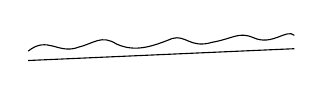
\begin{tikzpicture}[x=1cm,y=1cm]
\draw (0,0) .. controls (.25,.20) and (.38,-.05) .. (.64,.05)
 .. controls (.84,.10) and (.93,.21) .. (1.12,.09)
 .. controls (1.36,-.02) and (1.58,.06) .. (1.83,.16)
 .. controls (2.00,.21) and (2.06,.03) .. (2.33,.11)
 .. controls (2.61,.16) and (2.67,.25) .. (2.86,.17)
 .. controls (3.10,.06) and (3.28,.29) .. (3.38,.20);
\draw (0,-.12)--(3.38,.03);
\end{tikzpicture}}
% L13–16
\uuline{Questions} 1) Soit $C$ comme plus haut. Déterminer \unsure{ttes} les façons possibles de \deleted{\unsure{réduire la|réduire le} \unsure{rang}} \inserted{\unsure{'obtenir|définir} \unsure{la|C}} $C$-hyperalgèbre \deleted{Hom} tordue $\operatorname{Hom}_A(C,C)$ à partir d'une sous-$A$-hyperalgèbre $U$
% L17–21
(libre de rang $p$ sur $A$). Déterminer les $U$ \deleted{pour lesquels} qui sont isomorphes à l'algèbre enveloppante restreinte d'une $p$-algèbre de Lie \inserted{sur $A$, qui est un module} libre de rang 1\,; d'une \inserted{telle} $p$-algèbre \deleted{qui} avec puissance $p^{\text{ième}}$ nulle
% archive sheet number: 18
\scanpage{20}
% L1–2
2) Déterminer les classes à \unsure{isomorphismes|isomorphisme} près d'espaces \deleted{fibrés} principaux homogènes sous $B$.

% L3, divider
\figure{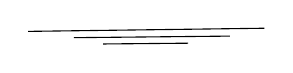
\begin{tikzpicture}\draw (0,0)--(3,.04) (.58,-.08)--(2.56,-.06) (.95,-.16)--(2.03,-.15);\end{tikzpicture}}

% L4–6
Soit $C$ une $A$-algèbre \inserted{libre de rang $p$}, munie d'une $A$-dérivation $D$ telle que $D^p=0$, et que les $D^i$ $(0\leq i\leq p-1)$ forment une \uline{base} de $\operatorname{Hom}_A(C,C)$ sur $C$.
% L7–8
Alors l'\uline{ensemble des éléments} \uline{de} $C$ \uline{annulés par} $D$ \uline{est $A$}. \deleted{\illegible{1}}
% slanted
\margin{autre \unsure{démonstration} : on étend les \unsure{scalaires} de $A$ à $C$.}
En effet, tout sous-$A$-module $M$ de $C$ qui est \inserted{libre de rang $m$ et} facteur direct \deleted{$\unsure{x}$} dans $C$,
% L10–12
est identique à l'ensemble $(M^\circ)^\circ$ des zéros de l'ens. $M^\circ$ des $v\in\operatorname{Hom}(C,C)$ qui s'annulent sur $M$ (\unsure{immédiat|évident}), et $M^\circ$ est un sous $C$-module libre de rang $p-m$ dans $\deleted{\unsure{C^p}}\operatorname{Hom}(C,C)$,
% L13–15
\deleted{\unsure{qui}} qui est facteur direct de ce sous-$C$-module\,; par suite\,; \uline{si}
% slanted
\margin{\uline{Lemme} à développer}
% L16–18
on a $p-m$ éléments $u_i$ dans $M^\circ$ qui \deleted{\unsure{engendrent un}} \inserted{forment la base d'un} sous-module \deleted{libre de rang \unsure{$p-m$} de \unsure{$K|C$}} \inserted{$L$ de $\operatorname{Hom}(C,C)$} qui est facteur direct,
% L19–21
alors nécessairement $L=M^\circ$, d'où $M=L^\circ$, i.e. $M$ est l'ens des éléments de $C$ annulés par les $u_i$. On applique ceci
% archive sheet number: 19
\scanpage{21}
% L1–2
à $M=A$, et aux $\unsure{u^i|u_i}=D^i$ $(1\leq i\leq p-1)$ \textendash\ on a $m=1$, etc \ldots

% L3–6
\deleted{S'il existe des} \deleted{\uline{Corollaire}}
\par\noindent\begin{tabular}{|p{.92\linewidth}}
Il existe dans $C$ un élément \deleted{\unsure{et un}} \inserted{$u$} \deleted{\unsure{qui}} tel que $Du=1$, et $u$ est unique à addition près d'un élément de $A$.
\end{tabular}

% L7–9
L'unicité résulte du fait qu'on a \deleted{$D^iu=0$ \unsure{pr tt} $i\geq2$, \unsure{donc, si $u'$ est comme $u$,}} \deleted{alors} $D^{\deleted{\unsure{i}}}(u-u')=0$ \deleted{\unsure{pour $i\geq1$}}, d'où $u-u'\in A$.

% L10–11
Montrons enfin que \deleted{\unsure{D}} l'on peut trouver $u$ avec $Du=1$.
% margin note written sideways
\margin{En effet, il existe \deleted{\unsure{un|tel}} un $A$-endomorphisme $\Theta$ de $C$ tel que $\Theta(1)=0$, et $\Theta(\unsure{x|u})=1$ ($x\in C$ \unsure{conven\textsuperscript{ble}}). On a $\Theta=\sum_{1\leq i\leq p-1}\lambda_iD^i=D\Theta'$, d'où $Du=1$, avec $u=\Theta'\unsure{x}$.}
% L11–13
\deleted{En effet, la question étant locale, on peut supposer} \deleted{$A$ \uline{local}. L'image de $D$ est alors un sous-$A$-module de $C$, isomorphe à}
% L14–16
\deleted{$C/\operatorname{Ker}D\simeq C/A$, donc \uline{libre} de rang $p-1$. Je dis qu'il \uline{contient} $A$, i.e. que $D(C)^{\circ}$ \unsure{est} contenu dans $A^\circ$, i.e que si}
% L17–19
\deleted{$v=\sum_{0\leq i\leq p-1}\lambda_i D^i$ est nul sur $D(C)^{\unsure{\circ|\infty}}$, alors $\lambda_0=0$ car la l'hypothèse sur $v$ signifie que $vD=0$, i.e. $\lambda_0=\lambda_1\ldots= \lambda_{p-2}=0$, O.K.}

% L20–21
\deleted{Si $x\in C$, \unsure{on}}
\uline{On a $\deleted{\unsure{C}}x^p\in A$ si $x\in C$} car $\deleted{\unsure{D(C^p}}\;Dx^p=0$.

% L22–23
\uline{Si} $u$ \uline{est} \deleted{comme plus \unsure{ht}} \inserted{tel que $Du=1$}, \uline{donc les} $u^i$ $(0\leq i\leq p-1)$ \uline{forment une} \uline{base} \uline{de} $C$ \uline{sur} $A$

% L24
\deleted{La \unsure{conclusion} \inserted{\unsure{question}} étant \uline{locale}, on peut supposer que}
% archive sheet number: 20
\scanpage{22}
% L1–6, one cancelled block
\deleted{$A$ est local. Montrons d'abord que les $u^i$ $(0\leq i\leq p-1)$ sont libres sur $A$. Soit en effet $\sum_0^{p-1}\lambda_i u^i=0$ une relation non-triviale entre les $u^i$, $(\lambda_i\in A)$, et soit $\lambda_\alpha$ le premier coéfficient non nul $(0\leq\alpha\leq p-1)$. Appliquant $D^\alpha$, on trouve $\unsure{\alpha!|\alpha}\,\lambda_\alpha\unsure{u|x}=0$, d'où $\lambda_\alpha=0$, absurde.}

% L7–8
Soit $u^p=a$, et soit $C'=A[\deleted{\unsure{X}}U]/(\deleted{\unsure{X}}U^p-a)$. \deleted{On \unsure{se trouve maintenant}} Soit $D'$ \inserted{une dérivation} dans $C'$ définie par $DU=1$, de sorte que $C'$ devient un espace homogène principal sous $B$ [cf ci-dessus]!
% L11–12
On a un hom \deleted{\unsure{qui}} $C'\mathrel{\unsure{\text{\textemdash}|\longrightarrow}}C$ défini $U\longrightarrow u$, et \deleted{\unsure{est}} c'est là un $B$-homomorphisme.

% L13–14
Il en résulte que \deleted{$C'\otimes C'\mathrel{\unsure{\longrightarrow|\simeq}} C\otimes C$ est} \inserted{$C'\mathrel{\text{\textemdash}} C$ est} un isomorphisme

% L15–18
[ de façon générale, si $E,E'$ sont des espaces fibrés principaux sous $G$, et \uline{si} on a un $G$-hom $E\mathrel{\text{\textemdash}}E'$, alors \deleted{\unsure{on en conclut tout de suite que|on en conclut tout de suite dans}} c'est un isomorphisme, pourvu que dans la catégorie $\unsure{\mathcal C|C}$, les \unsure{principes|diagramme} associés aux espaces à opérateurs marchent bien. Or
% L18–20, diagram between lines of the qualification
\diagram{\begin{tikzcd}[ampersand replacement=\&]
G\times E \arrow[r,dash] \arrow[d,"{\wr}"] \& G\times E' \arrow[d,"{\wr}"]\\
E\times E \arrow[r,"\sim"] \& E'\times E'
\end{tikzcd}}
% L21
\deleted{et d'autre part $E\times E\mathrel{\unsure{\text{\textemdash}|\longrightarrow}}E'\times E'$ est un}

% L22–24
C'est le cas si on se place dans la catégorie \margin{?}des anneaux finis sur $A$ \textendash\ [pourvu que $A$ soit noethérien ? \textendash\ ]
% archive sheet number: 21
\scanpage{23}
% L1–3
On a ainsi prouvé le

\uline{Théorème} $\unsure{H\!H|H^1}(A,B)$ s'identifie \deleted{à $A$} au groupe abélien
\par\noindent\begin{tabular}{|p{.92\linewidth}}
$A/A^p$ (où $A^p$ est l'ens des $x^p$, avec $x\in A$).
% L4–7
Si \deleted{\illegible{1}} $a\in A^{\deleted{\unsure{p}}}$, il lui correspond la classe de la $A$-algèbre $C_a=A[U]/(U^p-a)$, \unsure{muni|munie} de la $A$-dérivation $D_a$ définie par $D_aU=1$, et $C_a\simeq C_b$ si et \unsure{seult|seulement} si $a\equiv b$ $(A^p)$.

% L8–12
Soit $C$ un $B$-espace homogène principal, alors il existe dans $C$ un $u$ \deleted{\unsure{$\in A$|et}} tel que $Du=1$, et \deleted{\unsure{avec $a\in{}$ alors}} on a $u^p=a\in A$, $C\simeq C_a$ en \deleted{tant} que \deleted{fibré} $B$-fibré\,; $u$ est bien déterminé mod addition d'un élément de $A$.
\end{tabular}

% L13–15
On n'a pas prouvé que la loi additive naturelle de $H\!H(A;B)$ correspond à celle de $A/A^p$, mais ça ne peut être que facile.

% L16–19
\uline{Corollaire} Soit $C$ une $A$-algèbre commutative. Pour
\par\noindent\begin{tabular}{|p{.92\linewidth}}
\deleted{sur laquelle} \inserted{qu'il} existe \deleted{une} sur $C$ une structure de fibré \inserted{hom.} principal sous $B$, il faut et il suffit que $C$ ait une $p$-base sur $A$ réduite à un élément, \unsure{eh|et} i.e. un $u\in C$
% L20–22
tel que les $u^i$ $(0\leq i\leq p-1)$ forment une base de $C$ sur $A$. La donnée d'une telle structure de $B$-fibré \inserted{hom.} principal sur $C$
\end{tabular}
% archive sheet number: 22
\scanpage{24}
% L1–4
\par\noindent\begin{tabular}{|p{.92\linewidth}}
équivaut à la donnée d'une classe de tels $u$ mod addition d'un élément de $A$, i.e. à la donnée d'un élément de $C/A$ tel que, si $u$ en est un représentant, $(u)$ forme une $p$-base de
% L5–8
$C$ sur $A$\,; choisi $u$, la structure correspondante \deleted{\unsure{est}} est définie par la $A$-dérivation $D$ de $C$ telle que $Du=1$, et inversement, donné $D$, $u$ est \unsure{déterminé|déterminée} (mod $A$) par la condition $Du=1$.

% L9–12
Enfin, la donnée d'une \deleted{restriction des scalaires} \inserted{sous-$A$-hyperalgèbre} \inserted{$\unsure{U'|B'|\mathcal U'}$} de la $C$-hyperalgèbre tordue $\operatorname{Hom}_A(C,C)$, telle que \deleted{$\unsure{\operatorname{Hom}_A}$} $C$ devienne \deleted{\unsure{fibré}} homogène principal sous $U'$ et que $U'\simeq B$ \textendash\ équivaut à
% L13–16
la donnée d'une \deleted{\unsure{$x\in C$ $p$-base sur|$x\in C$ $p$-base de $u$}} \inserted{classe de} $p$-bases $(u)$ réduites à un élément $u$, en mettant dans la $=$ classe que $u$ les éléments $v=au+b$, avec $a\in A^*$ (unités de $A$) et $b\in A$\,; i.e.
% L17–20
l'ens de ces données est en correspondance biunivoque avec les éléments de l'espace \inserted{projectif} $\unsure{\mathbb P|P|\mathbf P}_A(C/A)=(C/A)/A^*$ associé au $A$-module $C/A$.
\end{tabular}
% archive sheet number: 23
\scanpage{25}
% L1
Autre façon d'obtenir ce résultat, et des résultats \uline{globaux}

% L2–4
Soit $X$ un \deleted{schéma} \inserted{préschéma} sur $\mathbb Z/p\mathbb Z$ ($p$ un nb premier). On a sur $X$ une suite exacte de schémas de groupes commutatifs
% L5
\diagram{\begin{tikzcd}[ampersand replacement=\&,column sep=small]
0\arrow[r] \& \mathcal B_X\arrow[r] \& G_{aX}\arrow[r,"\Phi"] \& G_{aX}\arrow[r] \& 0
\end{tikzcd}}
\margin{$\Phi=\text{Frobénius}$}
% L6–7
$G_{a,X}$ correspond à l'hyperalgèbre $\underline O[T]$ munie de $\Delta T=T\otimes1+1\otimes T$. \deleted{$\unsure{G}$}

% L8–11
L'hom de \unsure{frobénius|frobéneius|Frobenius} sur cette hyperalgèbre est donné par
\diagram{\begin{tikzcd}[ampersand replacement=\&]
\underline O[T] \& \underline O[T]\arrow[l,"{\varphi}"']
\end{tikzcd}}
\deleted{\unsure{associant}}
\[
\Phi(T)=T^p
\]
% L12–16
[on vérifie \deleted{\unsure{tout}} de suite que c'est compatible avec $\Delta$]. Son ``noyau'' est le sous-schéma de $G_{a,X}$ ``image inverse'' par $\Phi$ de la section unité de $G_{aX}$, \deleted{\unsure{par}} i.e. correspond au quotient $\underline O[T]/\Phi(\operatorname{Ker}\varepsilon)$
% L17–20
où $\varepsilon$ est l'augmentation dans $\underline O[T]$, donc ce noyau est bien $\underline O[T]/T^p\underline O[T)$ (car $\operatorname{Ker}\varepsilon$ est engendré par $T^p$). Je dis enfin que \deleted{$G$} $\Phi\colon G_{aX}\mathrel{\unsure{\text{\textemdash}|\longrightarrow}}G_{aX}$ est \uline{surjectif}
% zigzag in lower left margin
\reversemarginpar\margin{\figure{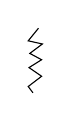
\begin{tikzpicture}\draw (0,0)--(-.13,-.16)--(.05,-.2)--(-.11,-.32)--(.04,-.4)--(-.12,-.5)--(.04,-.61)--(-.13,-.74)--(-.07,-.82);\end{tikzpicture}}}\normalmarginpar
% archive sheet number: 24
\scanpage{26}
% L1–6
\unsure{au|en|en un} sens technique suivant : Tout $X$-hom $G_{a,X}\mathrel{\longrightarrow}Y$ (où $Y$ est un préschéma sur $X$) qui est un $G_{a,X}$ hom (qud $G_{aX}$ opère sur le premier facteur grâce à $\Phi$, et sur $Y$ trivialement) est une \uline{section} de $Y$, i.e. se factorise en
\diagram{\begin{tikzcd}[ampersand replacement=\&]G_{aX}\arrow[r,"\mathrm{proj}"'] \& X\arrow[r] \& Y.\end{tikzcd}}
% L7–10
Cela se voit p.ex. sur le \deleted{fait que} \inserted{l'hom} d'\unsure{hyperalg.|hyperalgèbres} $\Phi$, en \unsure{notant|constatant|montrant} que celui-ci est injectif \margin{?}[du moins si $Y$ est affine\,; \deleted{\unsure{on peut}} \inserted{on peut} se ramener \unsure{tjrs} à ce cas].

% L11–12
% slanted
\margin{à justifier \unsure{théoriquement} ?}
On en conclut que l'on a \deleted{\unsure{que l'on a}} \inserted{une} suite exacte de cohomologie, qui s'écrit
% L13, cancelled beginning
\diagram{\begin{tikzcd}[ampersand replacement=\&,column sep=small]
\deleted{0}\arrow[r]\arrow[rr,dash,start anchor=west,end anchor=east,shift left=.35ex] \& \deleted{A[T]/T^p}\arrow[r]\arrow[loop above,draw=none,"{\rightarrow}"{description}] \& {}
\end{tikzcd}}
% L14
\diagram{\begin{tikzcd}[ampersand replacement=\&,column sep=4pt,font=\scriptsize]
0\arrow[r] \& H^0(X,\mathcal B_X)\arrow[r] \& A\arrow[r,"{\deleted{\unsure{x}}F}"] \& A\arrow[r] \& \unsure{H^1|H\!H}(X,B_X)\arrow[r] \& H^1(\unsure{Y|X},\underline O_X)\arrow[r,"F"] \& H^1(\unsure{X|Y},\underline O_X)
\end{tikzcd}}
% L15–18
[ ici $\Phi$ provient de Frobénius \deleted{\unsure{F}} \unsure{, et on|, est} \unsure{met|a mis} pour $A\colon H^0(X,\underline O_X)$ ] d'où $H^1(X,B_X)$ comme extension d'un \deleted{$A/A^p$} sous-groupe \deleted{\unsure{sous-groupe de}} \inserted{de $H^1(X,\underline O_X)$} par $A/A^p$. Si p.ex.
% L19–20
$X$ est une variété complète sur un corps algébriquement clos, alors on obtient pour
% archive sheet number: 25
\scanpage{27}
% L1–3
$\unsure{H^1|H\!H}(X,B_X)$ le sous-espace vectoriel de l'espace de dim finie $H^1(X,\underline O_X)$, \deleted{\unsure{an|annulé}} noyau de Frobenius.

% L4–7
\uline{Remarques} Soit $A=k[[X]]$, où $k$ est un corps algébriquement clos. Les revêtements \uline{non} triviaux \margin{\unsure{les|ses}} \deleted{ramifiés} de $A$ obtenus par extraction d'une racine $p$ième de $A$ sont \unsure{essentiellement|essentielt} isomorphes
% L8–9
[à condition de changer l'uniformisante, au besoin] à
\[
A[X^{n/p}]\simeq A[T]/(T^p-X^n)
\]
% L10–13
où $\unsure{1|0}\leq n\leq p-1$ \deleted{\unsure{si}} [pour $n=0$, on obtiendrait $\simeq A[T]/T^pA[\unsure{t|T}]$]. Si $n=1$, c'est un anneau local régulier. Sinon, il ne l'est pas, comme on voit facilement.

% L14–16
Par exemple, si $p=3$, \deleted{\unsure{si $A$}} et si on prend $n=\unsure{2|1}$, on trouve
\[
A[T]/(T^{\unsure{3|2}}-X^2)\simeq A[X^{2/3}],
\]
% L17–21
qui est isomorphe au sous-anneau de $\deleted{\unsure{B=}}k[[Y]]=k[[X^{1/3}]]$ formé des séries formelles dont le coefficient de $Y$ est nul. Pourtant, du point de vue de la théorie des $B$-\deleted{fibrés}\inserted{revêtements},
% archive sheet number: 26
\scanpage{28}
% L1–4
le revêtement envisagé est la somme de deux revêtements réguliers, correspondants \inserted{resp.} à l'adjonction d'une racine $p$ième de $X$, et de $-X+X^2$\,;
% L5–9
mais le produit fibré de ces deux anneaux \inserted{$C_1,C_2$} sur $A$ est déjà un anneau non régulier [car isomorphe à $C_1[T]/(T^p)\deleted{\unsure{a}}$, qui a des \unsure{élémts|éléments} nilpotents]
% archive sheet number: 27
